\section{商空间续论}
\sourcepage{261--262}
第 2.8 节已回顾商空间理论的一些方面，现在进一步讨论，特别考察其分离公理。商空间的分离性质通常表现不好；一般很难保证比 $T_1$ 更强的分离性，甚至 Hausdorff 性也常不易验证。下面给出三种可保证商空间为 Hausdorff 空间、事实上为正规空间的情形。

\entry{定理}{4.11.1}若商映射 $p:X\to Y$ 是闭映射，且 $X$ 正规，则 $Y$ 正规。

\textbf{证明：}因 $X$ 的单点集闭，闭映射将它映为 $Y$ 的闭单点集，故 $Y$ 为 $T_1$ 空间。设 $A,B\subset Y$ 为不交闭集，在 $X$ 中取不交开集 $U,V$，分别包含 $p^{-1}(A),p^{-1}(B)$。像集 $p(U),p(V)$ 不一定开，也不一定不交（图 4.11.1）。改令 $C=X\setminus U$、$D=X\setminus V$，则 $p(C),p(D)$ 闭。
\begin{center}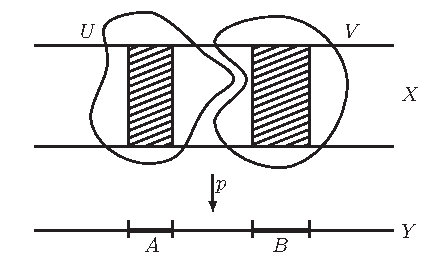
\includegraphics[width=.65\textwidth]{figures/4-11-1.pdf}\\图 4.11.1\end{center}
因为 $U\cap V=\varnothing$，De Morgan 定律给出 $C\cup D=X$，从而 $p(C)\cup p(D)=Y$，于是 $Y\setminus p(C)$ 与 $Y\setminus p(D)$ 不交。又因 $C$ 与 $p^{-1}(A)$ 不交，$p(C)$ 与 $A$ 不交，所以前者包含 $A$；同理后者包含 $B$。这就是所需的不交开邻域。\hfill$\square$

若 $X^*$ 是 $X$ 到闭集的一个分划，且商映射 $p:X\to X^*$ 闭，经典上称之为 $X$ 的\textbf{上半连续分解}（upper semicontinuous decomposition）。具体地，即每个闭集 $A\subset X$ 的\textbf{饱和集} $p^{-1}p(A)$ 都闭。此时 $X$ 正规蕴含 $X^*$ 正规。

\sourcepage{263}
\entry{定义}{4.11.2}设 $X,Y$ 不交，$A\subset X$ 闭，$f:A\to Y$ 连续。先给 $X\cup Y$ 赋拓扑和拓扑，再对每个 $y\in Y$，把 $\{y\}\cup f^{-1}(y)$ 压缩为一点，$X\setminus A$ 中的点保持各自独立。所得商空间记为 $X\cup_fY$，称为由 $f$ 决定的\textbf{粘合空间}（adjunction space），见图 4.11.2。
\begin{center}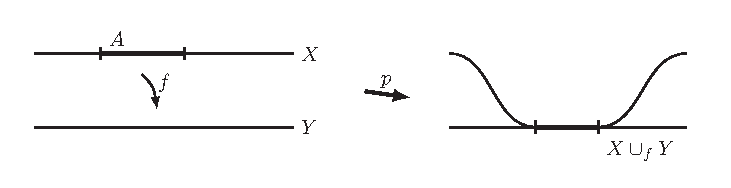
\includegraphics[width=.96\textwidth]{figures/4-11-2.pdf}\\图 4.11.2\end{center}
设商映射为 $p$。它把 $Y$ 同胚地映到商空间的闭子空间：限制 $p|_Y$ 连续且单射；若 $C\subset Y$ 闭，则 $f^{-1}(C)$ 在 $A$ 中闭，因 $A$ 闭而在 $X$ 中闭，所以 $p^{-1}p(C)=C\cup f^{-1}(C)$ 在拓扑和中闭。由商拓扑定义，$p(C)$ 闭。因此 $p|_Y$ 是到闭子空间 $p(Y)$ 的同胚。通常把 $Y$ 与该像认同。

若 $X,Y$ 为 $T_1$ 空间，每个等价类都闭，故 $X\cup_fY$ 也是 $T_1$ 空间。但 $p$ 通常不是闭映射，不能直接应用上一定理得到更强分离性。不过仍有如下结果。

\entry{定理}{4.11.3}若 $X,Y$ 正规，则 $X\cup_fY$ 正规。

\textbf{证明：}设 $B,C$ 为粘合空间中不交闭集，记
\[
B_X=p^{-1}(B)\cap X,\quad C_X=p^{-1}(C)\cap X,\quad
B_Y=p^{-1}(B)\cap Y,\quad C_Y=p^{-1}(C)\cap Y.
\]
\sourcepage{264}
由 Urysohn 引理，可取连续 $g:Y\to[0,1]$，在 $B_Y$ 上为 $0$、在 $C_Y$ 上为 $1$。因此 $gf$ 在 $A\cap B_X$ 上为 $0$、在 $A\cap C_X$ 上为 $1$。在闭集 $A\cup B_X\cup C_X$ 上定义 $h$：在 $A$ 上等于 $gf$，在 $B_X$ 上为 $0$，在 $C_X$ 上为 $1$。各部分定义相容，由闭集粘贴引理连续。再由 Tietze 延拓定理延拓为 $k:X\to[0,1]$。
\begin{center}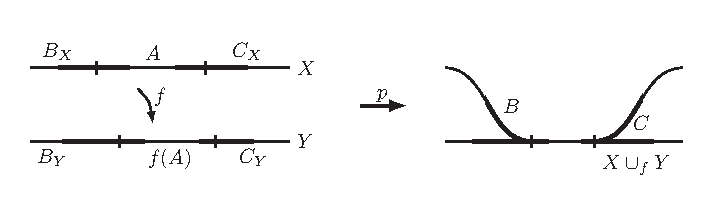
\includegraphics[width=.96\textwidth]{figures/4-11-3.pdf}\\图 4.11.3\end{center}
在拓扑和上定义 $\ell$，使其在 $X$ 上为 $k$、在 $Y$ 上为 $g$。它连续，且在每个等价类上为常值，因为 $k(a)=g(f(a))$。因此诱导商空间上的连续函数，在 $B$ 上为 $0$、在 $C$ 上为 $1$，说明空间正规。\hfill$\square$

我们已定义空间拓扑与子空间族协调的含义。现在稍加推广：给定拓扑空间族 $\{X_\alpha\}$，但其并集 $X$ 尚无拓扑。何时可在 $X$ 上赋予拓扑，使每个 $X_\alpha$ 保持原有子空间拓扑，且 $X$ 与这些子空间协调？

\entry{引理}{4.11.4}设集合 $X=\bigcup X_\alpha$。
\begin{enumerate}[label=(\alph*)]
\item 若已有一个底集为 $X$ 的拓扑空间 $X_T$，使所有 $X_\alpha$ 是其子空间，则可在 $X$ 上赋予与诸 $X_\alpha$ 协调的拓扑，且仍保持各子空间的原拓扑。这个拓扑一般比 $X_T$ 更细。
\item 若每个 $X_\alpha\cap X_\beta$ 在两者中都闭，且从两者继承的拓扑相同，则 $X$ 存在与诸 $X_\alpha$ 协调的拓扑；每个 $X_\alpha$ 在该拓扑中闭。
\end{enumerate}

\sourcepage{265}
\textbf{证明：}(a) 定义 $X_C$ 的闭集为所有满足 $A\cap X_\alpha$ 在 $X_\alpha$ 中闭的集合 $A$。这类集合对任意交及有限并封闭，且含空集和全集，故定义拓扑。若 $A$ 在 $X_T$ 中闭，它与每个子空间相交均闭，故也在 $X_C$ 中闭，因此后者更细。

要证每个 $X_\alpha$ 保持其子空间拓扑，只需比较闭集。一个 $X_C$ 中闭集与 $X_\alpha$ 的交按定义闭。反过来，若 $B\subset X_\alpha$ 闭，因它原是 $X_T$ 的子空间，可写 $B=A\cap X_\alpha$，其中 $A$ 在 $X_T$ 中闭，也在 $X_C$ 中闭。因此两种拓扑相同，协调性随即由定义成立。

(b) 仍用同样规则定义 $X_C$。若 $B$ 在 $X_\alpha$ 中闭，对任意 $\beta$，
\[
B\cap X_\beta=B\cap(X_\alpha\cap X_\beta)
\]
在交空间中闭；因交空间在 $X_\beta$ 中闭且两边继承拓扑相同，它在 $X_\beta$ 中闭。因此 $B$ 本身在 $X_C$ 中闭。\translatornote{原书上述等式右端首个集合误印为 $X$，应为 $B$。}这既说明子空间拓扑不变，也说明各 $X_\alpha$ 闭，完成证明。\hfill$\square$

\entry{例}{4.11.5}若 $K$ 是 $E^J$ 中的复形，则 $|K|$ 先有从 $E^J$ 继承的拓扑，其中每个单形均为子空间。由引理 (a)，还可赋予与所有单形协调的拓扑，它一般更细。这是第 1.3 节直接证明过的事实。

一般而言，即使各 $X_\alpha$ 有良好的分离性质，协调拓扑也未必保留这些性质。但对可数个闭子空间之并，可得如下定理。

\sourcepage{266}
\entry{定理}{4.11.6}若 $X$ 是可数个正规闭子空间 $X_i$ 之并，且拓扑与它们协调，则 $X$ 正规。

\textbf{证明：}每个点 $p$ 的单点集与每个 $X_i$ 相交均闭，故在 $X$ 中闭，$X$ 为 $T_1$ 空间。设 $A,B$ 为不交闭集，令 $Y_0=A\cup B$，$Y_n=X_1\cup\cdots\cup X_n\cup A\cup B$。在 $Y_0$ 上定义连续函数 $f_0$，在 $A$ 上为 $0$、在 $B$ 上为 $1$。

归纳延拓：$Y_n\cap X_{n+1}$ 在正规空间 $X_{n+1}$ 中闭，故用 Tietze 定理将 $f_n$ 在此交集上的限制延拓为 $g:X_{n+1}\to[0,1]$。由于 $Y_n$ 与 $X_{n+1}$ 在 $Y_{n+1}$ 中均闭，$f_n,g$ 可粘贴为连续的 $f_{n+1}$。所有 $f_n$ 合成 $f:X\to[0,1]$，仍在 $A,B$ 上分别为 $0,1$。它在每个 $X_n$ 上连续，由协调拓扑性质在 $X$ 上连续，故 $X$ 正规。\hfill$\square$

\entry{定义}{4.11.7}若空间的拓扑与其所有紧子空间协调，则称该空间\textbf{紧生成}（compactly generated）。这个定义用于习题 3。

\subsection*{习题}
\begin{enumerate}
\item 设 $X=\bigcup X_\alpha$，且每个交集 $X_\alpha\cap X_\beta$ 从两者继承相同拓扑。
\begin{enumerate}[label=(\alph*)]
\item 若所有交集在两边均开，证明 $X$ 上存在使诸 $X_\alpha$ 都成为子空间的拓扑。
\item 证明一般情况下，这样的拓扑未必存在。〔提示：取实数轴中不交稠密集 $A,B$，使其并的补集也稠密。令 $A,B,X_1=\R\setminus A,X_2=\R\setminus B$ 均继承实数轴的拓扑，$X_3=A\cup B$ 则取 $A,B$ 的拓扑和。令 $X=X_1\cup X_2\cup X_3$，考察 $\overline A$。〕
\end{enumerate}
\item 回忆 $\R^\infty=E^J$，其中 $J$ 为正整数集，每个 $\R^n\times\{0\}$ 都是其子空间。证明
\[
f:\R^\infty\to\R,\qquad f(x)=\sum_{i=1}^{\infty}ix_i
\]
在通常的度量拓扑中不连续，但在与诸 $\R^n\times\{0\}$ 协调的拓扑中连续。
\item 设 $X_C$ 为底集 $X$ 上与 $X$ 的所有紧子空间协调的拓扑。
\begin{enumerate}[label=(\alph*)]
\item 证明 $B\subset X$ 在从 $X$ 继承的拓扑中紧，当且仅当在从 $X_C$ 继承的拓扑中紧。〔提示：还要证明这两个子空间拓扑实际上相同。〕
\item 证明 $X_C$ 紧生成，从而 $(X_C)_C=X_C$。
\item 证明恒等包含 $X_C\to X$ 诱导奇异同调同构。
\item 记 $X\times_CY=(X\times Y)_C$。证明对复形 $K,L$，$|K|\times_C|L|$ 的拓扑与所有 $\sigma\times\tau$（$\sigma\in K,\tau\in L$）协调。与第 2.8 节习题 6 比较。〔提示：若 $D\subset X\times Y$ 紧，则 $D\subset A\times B$，其中 $A,B$ 紧。〕
\end{enumerate}
\item 证明定理 4.11.6 不适用于不可数族。〔提示：令 $[0,\omega_1]$ 为带最小元和最大元的不可数良序集，其中每个 $\alpha<\omega_1$ 的初段 $[0,\alpha]$ 可数。空间 $[0,\omega_1)\times[0,\omega_1]$ 不正规，见 [Mun00] 第 203 页例 2。〕
\item 寻找一个附加条件，使定理 4.11.6 对不可数并也成立。
\end{enumerate}
